\section{Resolving Ambiguities Using the Abstraction Tree}
\subsection{Resolving Context Ambiguities}
The abstraction tree not only contains
\begin{Verbatim}
Algorithm 1
function [HM]=eligible(HM_tree,Req)
BM = root of HM_tree
while (BM is not empty)
 For every model M in BM
  If (all behaviors in EnvB(Req) are not abstracted with other behaviors)
   Remove M from BM
   save M in HM
  else
   add children of M in BM
  endif
 endfor
endwhile
Return HM
\end{Verbatim}
%BM = all models in HM_tree with all Prop(Req)
%For all M in BM
 %while (in the parent of M no behavior in Prop(Req) is abstracted with other behaviors)
	 %M = parent of M
 %endwhile
 %save M in HM
 %endfor
\subsection{Resolving Validity Ambiguities}

\begin{Verbatim}
Algorithm 2
Input: system model PM, abstraction tree for environment HM_tree, requirement Req
Output: Counter examples CE and corresponding model refinements
[HM]=eligible(HM_tree,Req);
Mc= HM;
 while (Mc is not empty)
  For all M in Mc
   [satisfied,CE]=ModelChecking(M,PM,Req);
	 Remove M from Mc
	 If satisfied==0
	  add the children of M to Mc
		cache CE
	else
		save CE from the parent model
	endif
 endfor
endwhile
Return all saved CEs and their corresponding models
\end{Verbatim}



\section{Case Study: Closed-loop Model Checking of a Dual Chamber Pacemaker}
\subsection{Pacemaker Model}
\todo[inline]{We may not have space but if we do we should put the 5 timing cycle figure here}
\subsection{Heart Model Abstraction Tree}
We first develop a list of concrete heart models corresponding to common heart conditions. By systematcally applying rules from Section \ref{ruleBasedHeartModelAbstraction} we created an abstraction tree $HM\_tree$ for the heart (\figref{HM_abs}). Note that applying rules in different order results different abstraction tree. The order used to obtain $HM\_tree$ is based on the domain knowledge that certain heart conditions may have similar outputs to the pacemaker. This systematic grouping maintains the physiological-relevance of the heart model even at higher abstraction levels, and reduce the necessity to resolve ambiguities at lower abstraction levels when model checking certain requirements.
\begin{figure}[!t]
		\centering
		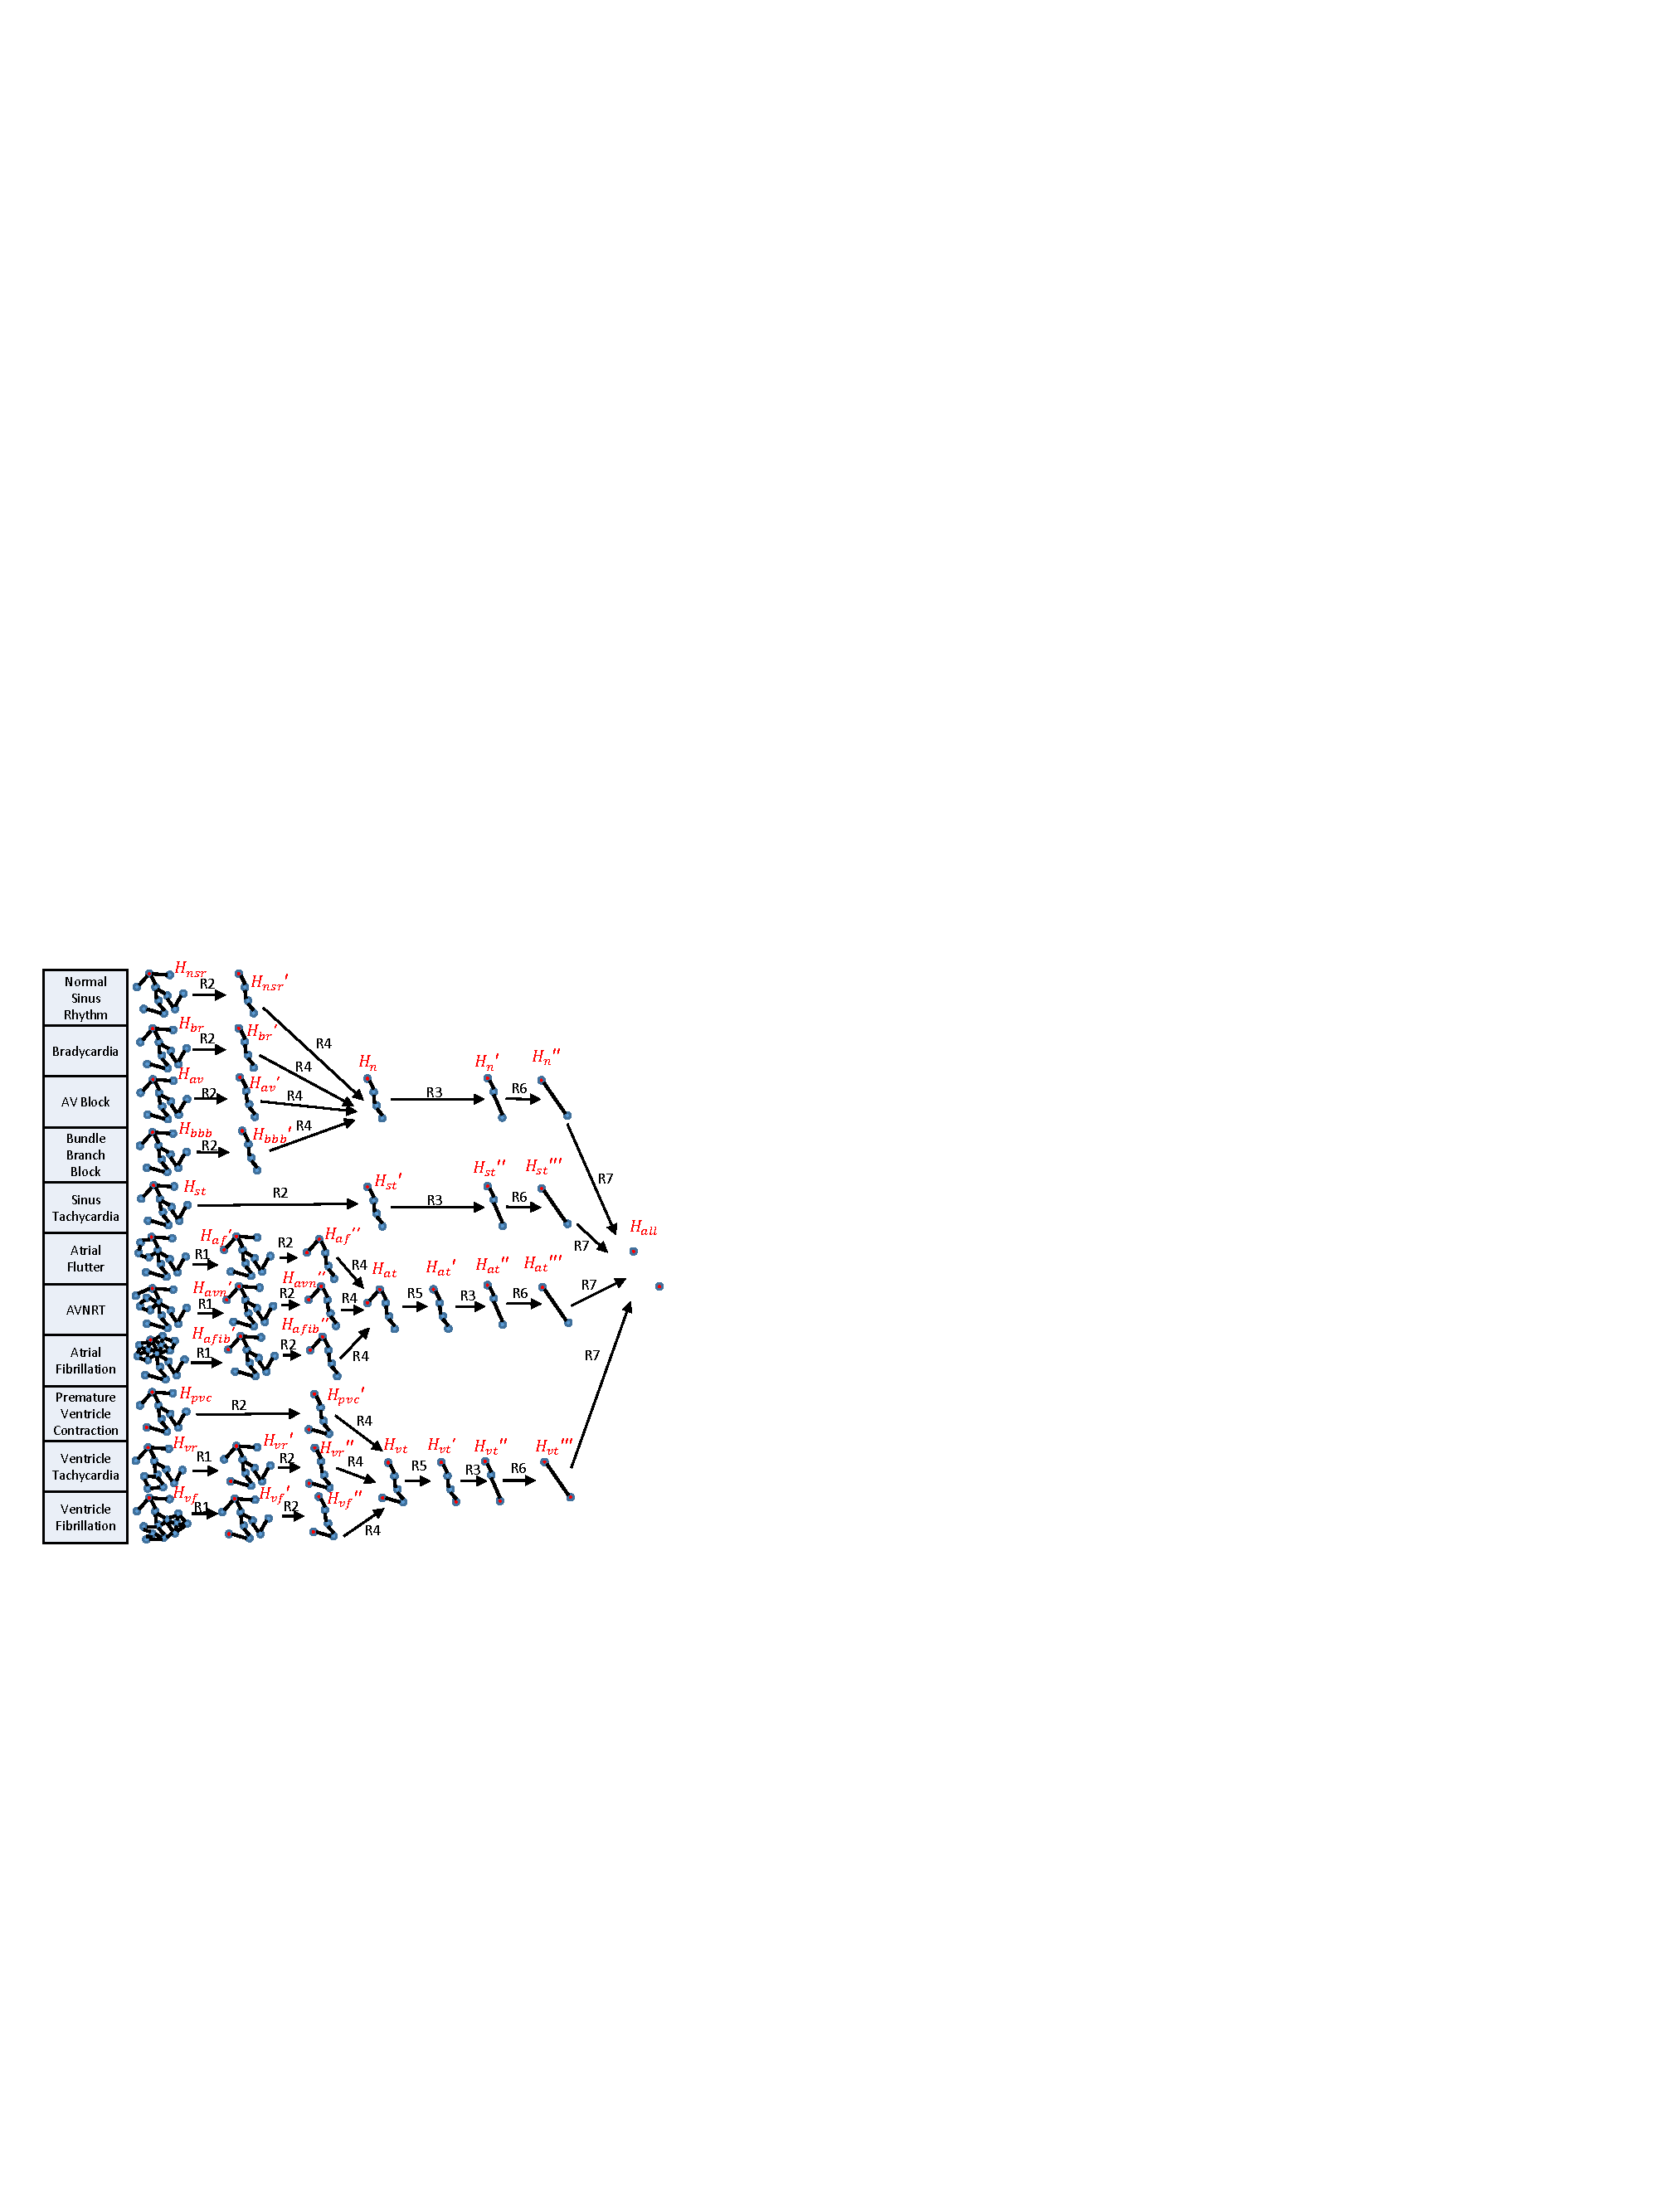
\includegraphics[width=0.9\textwidth]{figs/abs.pdf}
		%\vspace{-5pt}
		\caption{\small Heart Model Abstractions}
		  %\vspace{-15pt}
		\label{fig:HM_abs}
\end{figure}

Besides model structure changes, applying abstraction rules also merges the behaviors of the model, which is documented for each abstraction. Here we demonstrate the behavior merging process on a subset of the abstraction tree (\figref{abs_sim}). In $H_{vt}''$, we have self activation behavior $NA.self$ and $NV.self$ for node $NA$ and conduction behavior $NV$,$(NA,AV').cond$ and $(AV',NV).cond$ for path $(NA,AV')$ and $(AV',NV)$. After applying Rule 6 we obtain $H_{vt}''$ with
$$NA'.self=\{NA.self\},NV'.self=\{NV.self\}$$
$$(NA',NV').cond=\{AV'.block,(NA,AV').cond,(AV',NV).cond\}$$
After applying Rule 7 we obtain $H_{all}$ with:
$$NA''.self=\{NA.self,(NA',NV').cond\}$$
$$NV''.self=\{NV.self,(NA',NV').cond\}$$
These information on behavior abstractions are useful to determine whether a model is appropriate for a requirement.
\begin{figure}[!t]
		\centering
		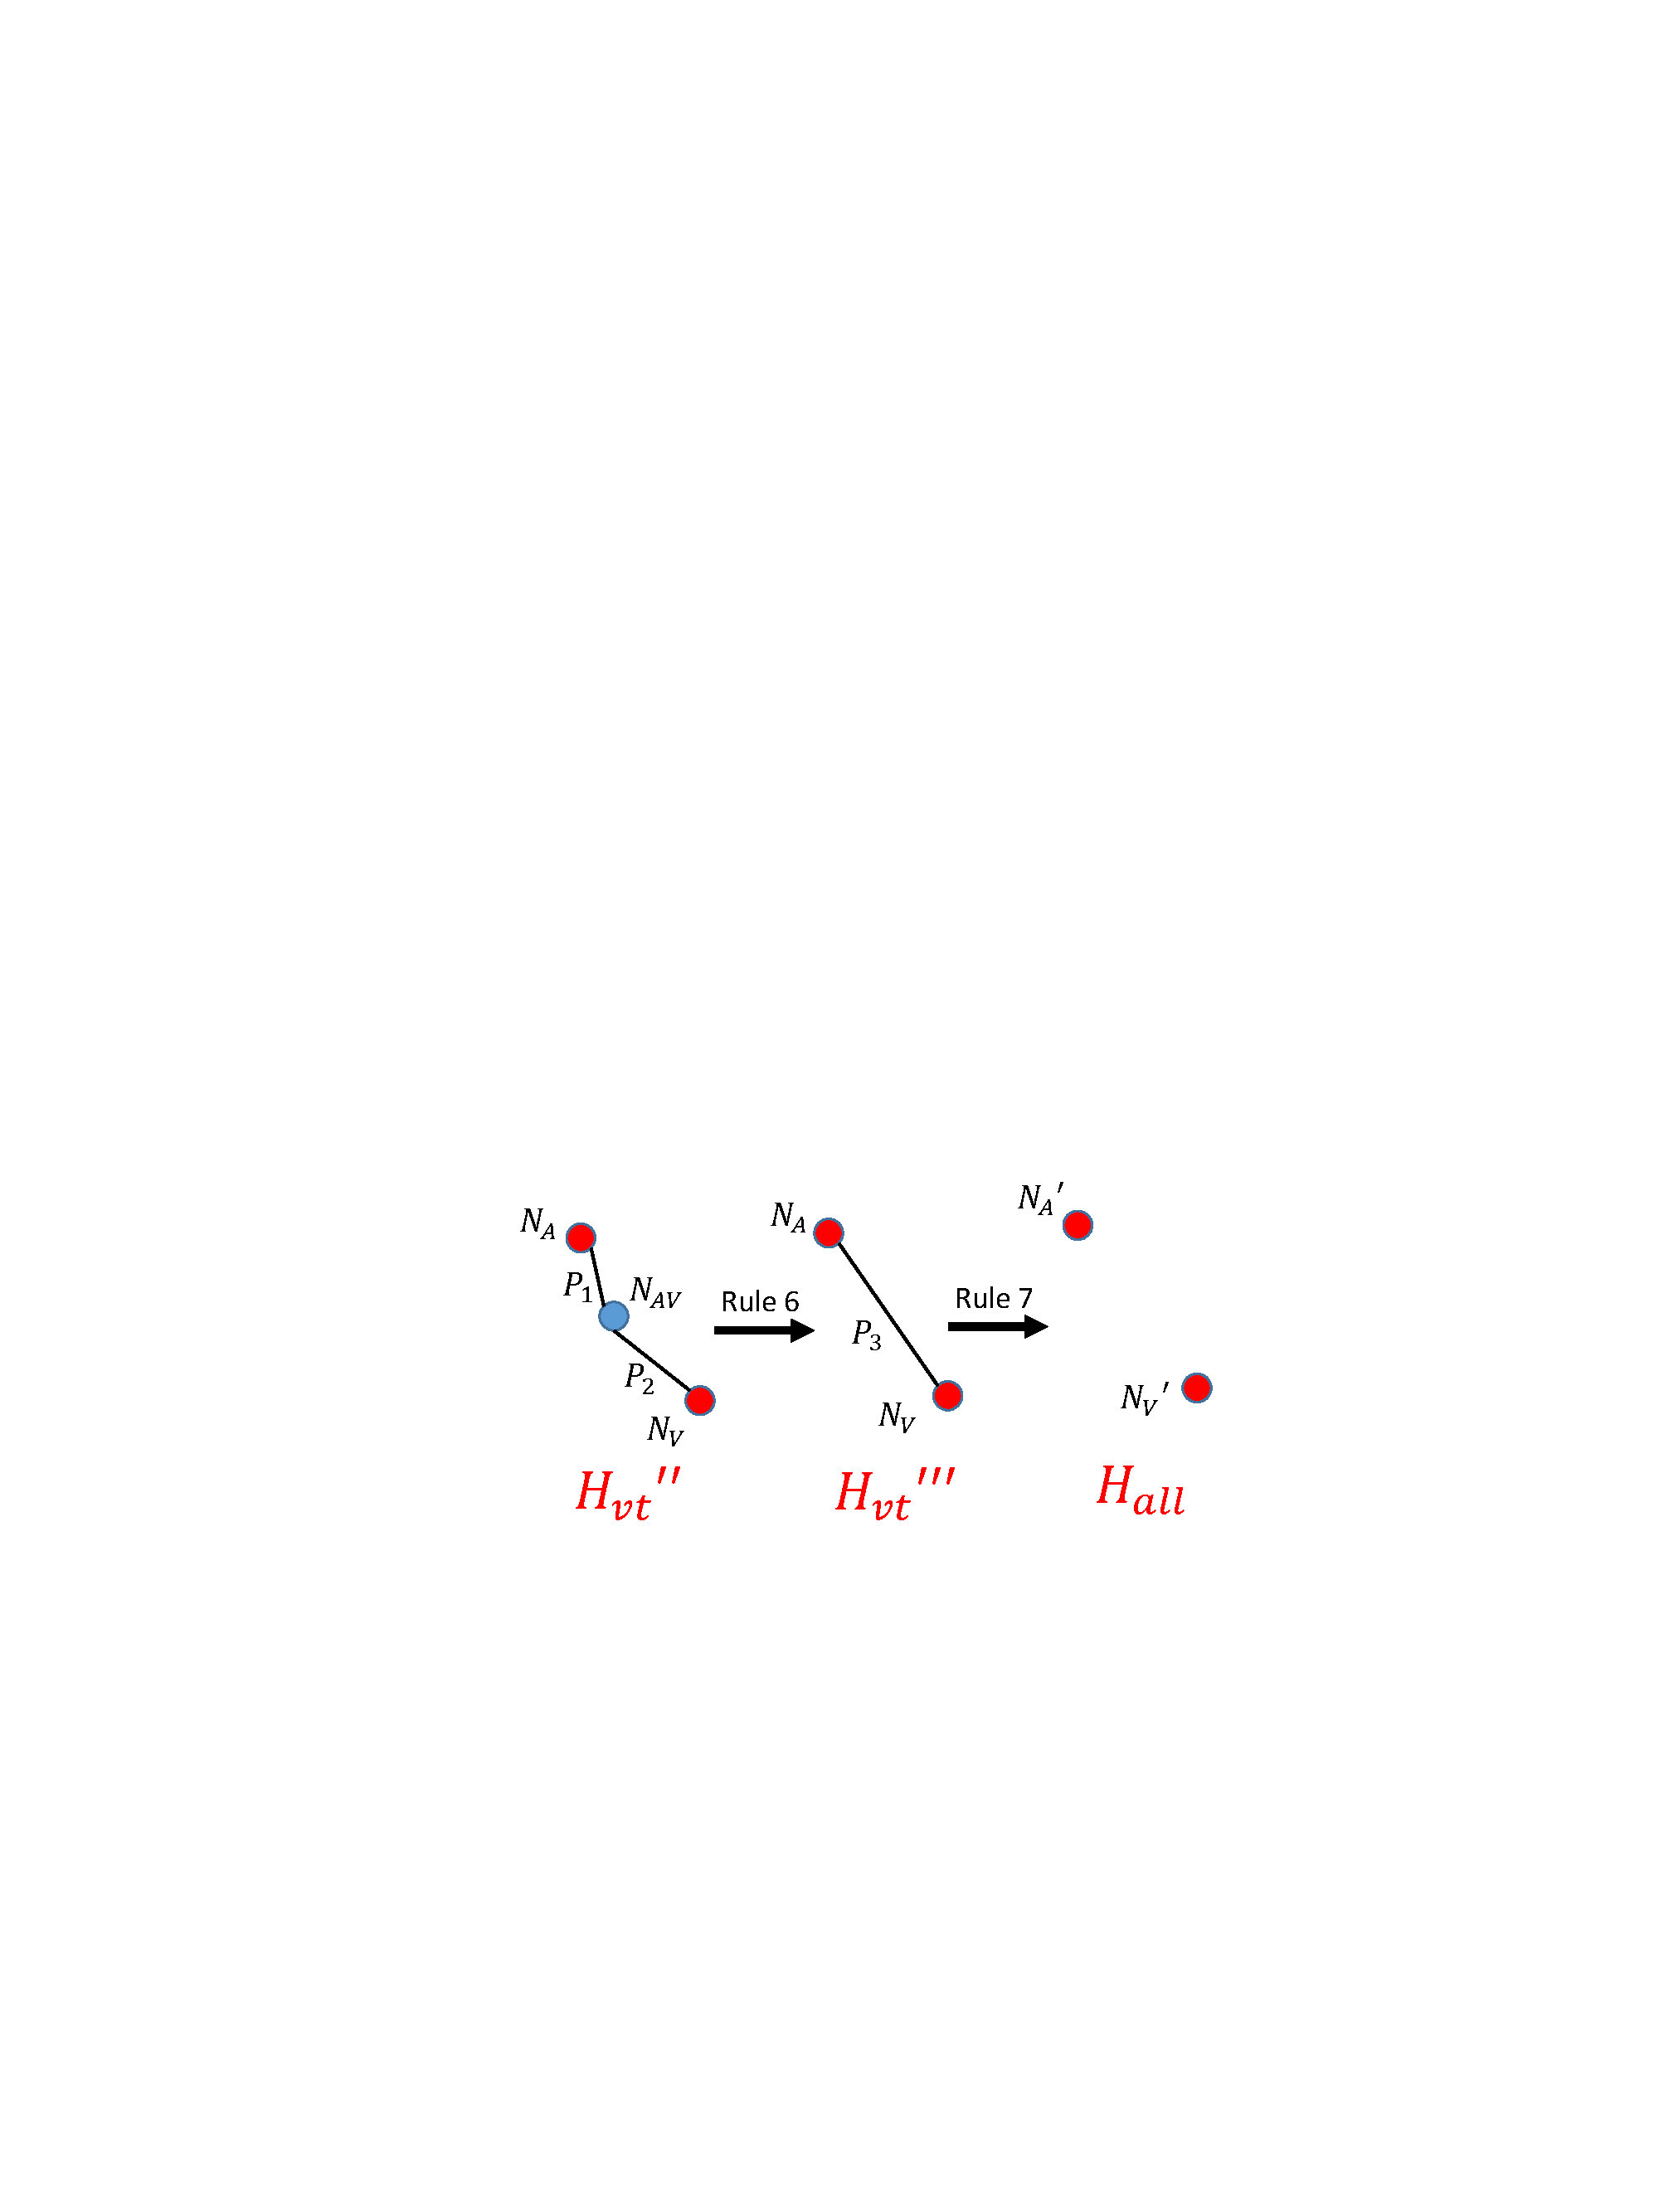
\includegraphics[width=0.5\textwidth]{figs/abs_sim.pdf}
		%\vspace{-5pt}
		\caption{\small Abstraction Example}
		  %\vspace{-15pt}
		\label{fig:abs_sim}
\end{figure}

\subsection{Requirement Encoding}
Physiological requirements can be automatically mapped to model behaviors and parameters. In general, a requirement has \emph{pre-conditions} under which the requirement should hold. The pre-conditions are open-loop physiological conditions which are in terms of constraints on model behaviors. The \emph{post-conditions} are closed-loop behaviors that the device should achieve. The requirement below is designed to prevent the pacemaker from pacing too fast.
\begin{itemize}
	\item Pre-condition: Atrial self-activation rate (60bpm - 200bpm)
    \item Post-condition: Intervals between ventricular paces should be no shorter than 500ms
\end{itemize}
\begin{figure}[!h]
		\centering
		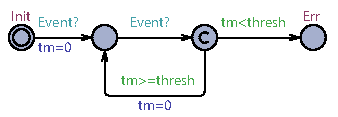
\includegraphics[width=0.4\textwidth]{figs/monitor.pdf}
		%\vspace{-5pt}
		\caption{\small monitor}
		  %\vspace{-15pt}
		\label{fig:monitor}
\end{figure}
With behavior mapping and a monitor (\figref{monitor}), the requirement can be translated to:
$$Req1: NA.self.min=300 \&\& NA.self.max=1000 \Rightarrow not M.Err$$
The environment behavior specified in $Req1$ is $EnvB(Req1)=NA.self$.
\subsection{Choosing Appropriate Heart Model For the Requirement}
To verify the closed-loop system with pacemaker model $PM$ and heart model abstraction tree $HM\_tree$ (\figref{abs_exam}) against requirement $Req1$, we start by searching for the most abstract appropriate models from the abstraction tree. We call the function specified in Algorithm 1: $[HM]=eligible(HM\_tree,Req1)$. At the root level heart model $H_{all}$, $NA.self$ is abstracted with $(NA',NV').cond$. As the result, $H_{all}$ is not appropriate for $Req1$. $NA.self$ is not abstracted with other behaviors in the children of $H_{all}$: $H_n'',H_{at}'''',H_{vt}'''$, thus these 3 heart models are outputted as the most abstract appropriate models for $Req1$.
\subsection{Providing Meaningful Counter-examples to the Physicians}
After we choose the appropriate models for $Req1$, we have: 
$$HM=\{H_n'',H_{at}'''',H_{vt}'''\}$$
Then we run Algorithm 2. By model checking on all 3 initial models in UPPAAL we have: 
$$[1,[]]=ModelChecking(H_n'',PM,Req1)$$
 $$[0,CE_1]=ModelChecking(H_{at}'''',PM,Req1)$$
$$[0,CE_2]=ModelChecking(H_{vt}''',PM,Req1)$$
The algorithm keeps going down the abstraction tree, and at certain intermediate step we have:
 $$[0,CE_a]=ModelChecking(H_{st}',PM,Req1)$$
  $$[0,CE_b]=ModelChecking(H_{pvc}',PM,Req1)$$
	$$[0,CE_c]=ModelChecking(H_{at},PM,Req1)$$
 $$[1,[]]=ModelChecking(H_{vr}'',PM,Req1)$$
 $$[1,[]]=ModelChecking(H_{vf}'',PM,Req1)$$

\begin{figure}[!t]
		\centering
		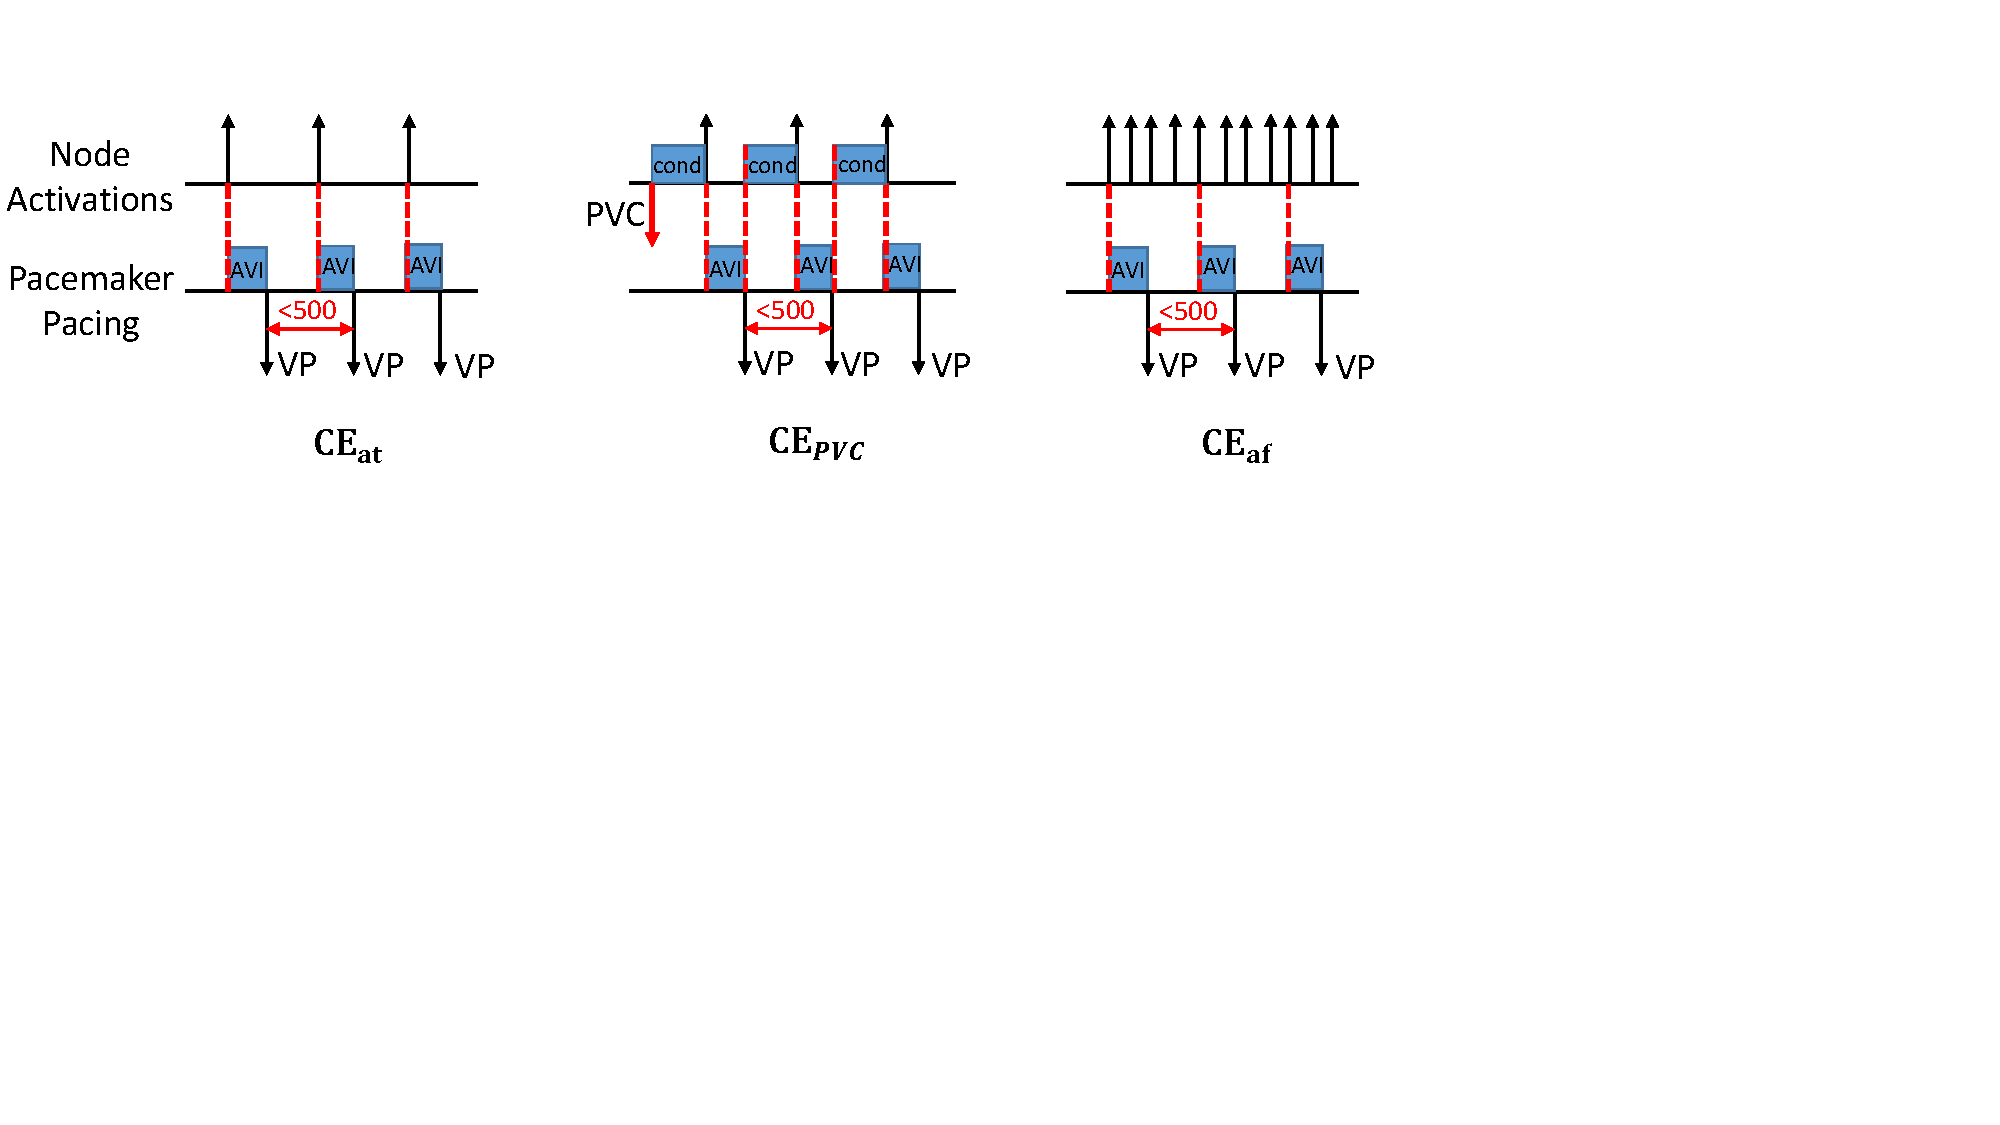
\includegraphics[width=0.9\textwidth]{figs/case.pdf}
		%\vspace{-5pt}
		\caption{\small Counter-examples}
		  %\vspace{-15pt}
		\label{fig:CE}
\end{figure}
The counter-examples from more refined models provide more detailed mechanism of the requirement violations, and distinguish the physiological conditions that can trigger the violations. It is much easier for the physician to determine the validity of the counter-example. The counter-examples from the example above are illustrated in \figref{CE}. $CE_a$ corresponds to fast intrinsic heart rate thus is a safe execution of the pacemaker. $CE_b$ corresponds to a scenario called Endless Loop Tachycardia during which the pacemaker and the heart forms a conduction loop that increases the heart rate inappropriately. In $CE_c$ the pacemaker extends fast atrial rate to more dangerous fast ventricular rate, which is referred to as Atrial Tachycardia Response of a pacemaker. Both $CE_b$ and $CE_c$ are inappropriate executions of the pacemaker .$CE_a$ and $CE_b$ can have the same input-output executions on the pacemaker side and can only be differentiated on the heart model side. After the physician examines the counter-example the programmer can work on debugging.
%$NA\_self$ is in $H_3$, we go one level up, in $H_4$ the behavior is not merged with any other parameters. In $H_5$ $NA\_self$ is merged with  $NA'-NV'.cond$ so $H_4$ is returned as the appropriate heart model for R1. In \cite{STTT13} we used $H_4$ to verify the correctness of the ELT termination algorithm. With a basic DDD pacemaker we have $H_4 || P_{DDD}\models R1$. The counter-example returned is exactly the ELT behavior. Then we implement the ELT termination algorithm and we have  $H_4 || P_{ELT}\not\models R1$, meaning ELT has been successfully terminated, and only the ELT is terminated. 
%
%\subsection{Inappropriate Model Refinements}
%If we follow the traditional CEGAR framework and verify the property using $H_5$, an abstract counter-example would return, which is shown in %\figref{C_amiguity}. However the counter-example correspond
 




